\documentclass{beamer}

\usepackage{amsmath}
\usepackage{mathtools}
\usepackage{amsfonts}
\usepackage{amsthm}
\usepackage{amssymb}
\usepackage{graphicx}
\usepackage{hyperref}

\usepackage{algpseudocode}
\usepackage{algorithm}

\makeatletter
\renewcommand{\ALG@beginalgorithmic}{\small}
\makeatother

%\usepackage{beamerthemeshadow}
\usetheme{Boadilla}
\title[data-microscopes]{
  \texttt{data-microscopes}: Bayesian non-parametric inference made simple in Python
}
\author{Stephen Tu}
%\institute{MIT CSAIL}
\date[SFPython]{SF Python - August 20, 2014}

\newtheorem{mydef}{Definition}
\newtheorem{mylemma}{Lemma}
\newtheorem{mythm}{Theorem}

\DeclareMathOperator*{\argmin}{arg\!\min}
\DeclareMathOperator*{\argmax}{arg\!\max}
\DeclareMathOperator*{\rank}{rank}
\newcommand{\dom}{\mathop{\mathrm{dom}}}
\newcommand{\pdf}{{\mathrm{pdf}}}
\newcommand{\Unif}{{\mathrm{Unif}}}

\newcommand{\A}{\ensuremath{\mathcal{A}}}
\newcommand{\X}{\ensuremath{\mathcal{X}}}
\newcommand{\Y}{\ensuremath{\mathcal{Y}}}
\newcommand{\Z}{\ensuremath{\mathcal{Z}}}
\newcommand{\R}{\ensuremath{\mathbb{R}}}
\newcommand{\Q}{\ensuremath{\mathbb{Q}}}
\newcommand{\N}{\ensuremath{\mathbb{N}}}
\newcommand{\F}{\ensuremath{\mathcal{F}}}
\newcommand{\Hyp}{\ensuremath{\mathcal{H}}}
\newcommand{\Loss}{\ensuremath{\mathcal{L}}}
\newcommand{\Cset}{\mathcal{C}}
\newcommand{\norm}[1]{\left\lVert #1 \right\rVert}
\newcommand{\onenorm}[1]{\left\lVert #1 \right\rVert_{1}}
\newcommand{\mb}[1]{\mathbf{#1}}
\newcommand{\ip}[2]{\ensuremath{\langle #1, #2 \rangle}}
\newcommand{\PD}[2]{\ensuremath{\frac{\partial #1}{\partial #2}}}
\newcommand{\D}[1]{\ensuremath{\frac{\partial}{\partial #1}}}
\newcommand{\Var}{\mathrm{Var}}
\newcommand{\Expect}{\mathbb{E}}
\newcommand{\abs}[1]{\ensuremath{\left| #1 \right|}}
\newcommand{\floor}[1]{\lfloor #1 \rfloor}
\newcommand{\ceil}[1]{\lceil #1 \rceil}
\newcommand{\G}{\mathcal{G}}
\newcommand{\BigO}{\ensuremath{\mathcal{O}}}
\newcommand{\Borel}{\mathcal{B}}

\begin{document}

\begin{frame}
\titlepage
\end{frame}

\section{Preliminaries}
\subsection{Definitions}

\begin{frame}
\frametitle{Why do we need yet another machine learning library?}
There are already many Python libraries out there which specialize to 
some area of machine learning:
\begin{itemize}[<+->]
  \item \texttt{scikit-learn}
  \item \texttt{pymc}
  \item \texttt{pybrain}
  \item \texttt{pystan}
  \item \texttt{shogun}
  \item Countless more (sorry if I missed yours)
\end{itemize}
\end{frame}


\begin{frame}
\frametitle{Why do we need yet another machine learning library?}
\begin{block}{Goal}
\emph{Do one thing well}: inference (via Markov Chain Monte Carlo)
for a fixed set of non-parametric models 
\end{block}

Doing it well means being \textbf{correct} and \textbf{fast}!
\end{frame}


\begin{frame}
\frametitle{Great, so what does it mean to be Bayesian and non-parametric?}
\begin{itemize}[<+->]
  \item \textbf{Disclaimer}: way too much to possibly cover in a short time!
  \item We'll focus on one specific problem: 
    given a set of points, find the most likely clustering.
  \item This will lead us to the \emph{Dirichlet process mixture model}.
\end{itemize}
\end{frame}


\begin{frame}
\frametitle{Dirichlet process mixture model}
\begin{itemize}
  \item Why not just $k$-means?
    \begin{equation*}
      \argmin_{C_1, ..., C_k} \sum_{i=1}^{k} \sum_{x_j \in C_i} \norm{ x_j - \mu_i }^2 \qquad \mu_i = \frac{1}{\abs{C_i}} \sum_{x_j \in C_i} x_j
    \end{equation*}
\end{itemize}
\end{frame}


\begin{frame}
\frametitle{Dirichlet process mixture model}
\begin{itemize}
  \item Picking the $k$ is annoying.
    \begin{figure}
    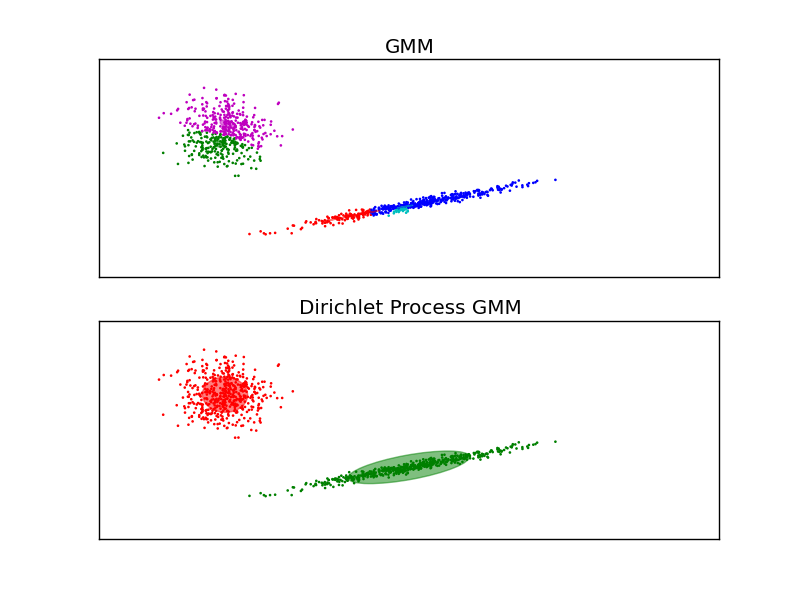
\includegraphics[scale=0.3]{images/plot_gmm_0011.png}
    \caption{\url{http://scikit-learn.org/stable/_images/plot_gmm_0011.png}}
    \end{figure}
\end{itemize}
\end{frame}


\begin{frame}
\frametitle{Dirichlet process mixture model}
\begin{itemize}
  %\item Why not just $k$-means?
  \item What if you have a \emph{model} of the data? E.g. you know the 
    data is from a mixture of gaussian distributions.

  \item What if there is no \emph{metric} on the data type? E.g. the data is
    categorical?
\end{itemize}
\end{frame}


\begin{frame}
\frametitle{Dirichlet process mixture model}
\begin{itemize}[<+->]
  \item The DPMM deals with these issues in a elegant mathematical framework.
  \item It is a probabilistic model which describes the generative process
    of $n$ i.i.d. observations $Y_1, ..., Y_n$ as:
    \begin{align*}
      G &\sim \text{DirichletProcess}(\alpha, H) \\
      \theta_i | G &\sim G \\
      Y_i | \theta_i &\sim F(\theta_i)
    \end{align*}
    where $F(\cdot)$ is a likelihood model (e.g. Gaussian),  $H(\cdot)$ is the
    \emph{prior} distribution (e.g. Normal-Inverse-Wishart) over the parameters
    of $F(\cdot)$, and $\alpha \in \R^{+}$ is chosen a-priori.
\end{itemize}
\end{frame}


\begin{frame}
\frametitle{Dirichlet process mixture model}
\begin{itemize}[<+->]
  \item The previous mathematical description is probably too abstract to mean
    anything at this point.

\end{itemize}
\end{frame}



\section{Conclusion}
\begin{frame}
\frametitle{Conclusion}
Thanks! Questions?
\cite{chaudhuri11}
\end{frame}

\begin{frame}[allowframebreaks]{References}
\small
\bibliographystyle{alpha}
\bibliography{p}
\end{frame}
\end{document}
